% Metódy inžinierskej práce

\documentclass[10pt,twoside,slovak,a4paper]{article}

\usepackage[slovak]{babel}
%\usepackage[T1]{fontenc}
\usepackage[IL2]{fontenc} % lepšia sadzba písmena Ľ než v T1
\usepackage[utf8]{inputenc}
\usepackage{graphicx}
\usepackage{url} % príkaz \url na formátovanie URL
\usepackage{hyperref} % odkazy v texte budú aktívne (pri niektorých triedach dokumentov spôsobuje posun textu)
\usepackage{graphicx}
%\usepackage{pdfpages}
%\usepackage{csvsimple}
\DeclareGraphicsExtensions{.png}

\usepackage{cite}
%\usepackage{times}


\pagestyle{headings}

\title{Časté chyby pri vývoji softvéru\thanks{Časté chyby pri vývoji softvéru, ak. rok 2020/21, vedenie: Vladimir Mlynarovic}} % meno a priezvisko vyučujúceho na cvičeniach

\author{Adam Melikant\\[2pt]
	{\small Slovenská technická univerzita v Bratislave}\\
	{\small Fakulta informatiky a informačných technológií}\\
	{\small \texttt{xmelikant@stuba.sk}}
	}

\date{\small 14. December 2021} % upravte



\begin{document}

\maketitle

\begin{abstract}
V tomto článku sa budeme zaoberať najčastejšími chybami, ktoré môžu nastať pri komplexnom vývoji akéhokoľvek typu softvéru. Celý tento vývoj rozdelíme na jednotlivé celky popisujúce postupy vývoja softvéru. Tieto celky podrobne rozoberieme a poukážeme na jednotlivé nedostatky, ktoré následne môžu spôsobovať závažné problémy v praxi. Začneme od začiatku: Plánovanie potrebných informácií, zdrojov, cielený účel softvéru, rozšírenia atď. Následne rozoberieme štruktúru softvéru, chyby pri navrhovaní, programovaní či celkovej štruktúre, návrhu a funkcionalite. Dostatočne vysvetlíme zaužívané postupy, ktoré vedú k najčastejším chybám a aj to ako sa im efektívne vyhnúť prípadne čo najrýchlejšie opraviť aby sa následne zamedzilo kaskádovému vzniku ďalších problémov. Po úspešnom dokončení softvéru poukážeme na chyby v distribúcií a rôznych iných aplikáciách, ktoré sú častým nedostatkom hlavne z hľadiska dosiahnutia čo najväčšieho dopytu.
\end{abstract}


\section{Úvod}
Každý plán vývoja softvéru je navrhnutý s ohľadom na finančné a časové obmedzenia dostupné pre zainteresované strany. Pravidelný výskyt chýb však môže viesť k zbytočným prieťahom v pláne. To môže spôsobiť nadmerné finančné zaťaženie a v najhoršom prípade odmietnutie produktu. Preto si vývojový tím musí byť vedomý bežných chýb, ktoré sa môžu počas procesu stať. Tu uvádzame niektoré bežné chyby, ktorým je potrebné sa vyhnúť, aby mohol pokračovať správny životný cyklus vývoja softvéru. % Opíšeme všetky fázy cyklu softvéru a zdôrazníme časté chyby, ktoré sa tam často vyskytujú.  
Diagram \ref{fig:D1} opisuje životný cyklus sú vyzačené fázy, v ktorých sa najčastejšie vyskytujú chyby.
\begin{figure}[h]
    \centering
    
\includegraphics[scale=0.35]{vyvoj_diagram.png}
    \caption{Životný cyklus softvéru.}
    \label{fig:D1}
\end{figure}

\pagebreak
Graf \ref{fig:D2} znázorňuje precentuálny výskyt chýb v rôznych fázach vývoja softvéru.

\begin{figure}[h]
    \centering
    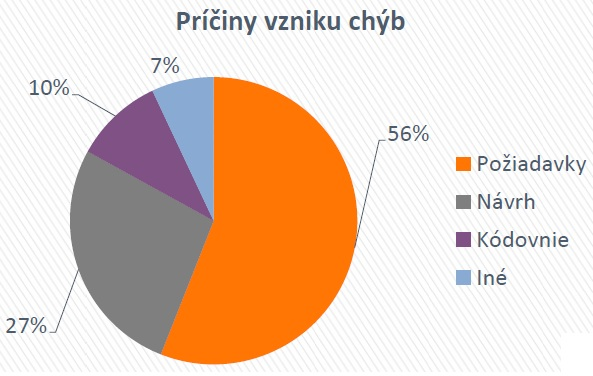
\includegraphics[scale=0.35]{priciny_chyb.jpg}
    \caption{Príčiny vzniku chýb pri vývoji softvéru, prevzaté zo zdroja \cite{VyvojProces}.}
    \label{fig:D2}
\end{figure}


\section{Počiatočný prieskum}
Testovanie vierohodnosti nápadov pred vývojom je kľúčovým krokom, ako sa vyhnúť uviaznutiu. V prvej fáze sa vývojári a tvorcovia nápadov stretnú a dosiahnu konsenzus ohľadom vlastností a funkčnosti programu. To zahŕňa aj brainstorming s odborníkmi z odvetvia o aktuálnych trhových trendoch a požiadavkách. 

Rozhodovanie o nákladových faktoroch je zároveň dôležitým faktorom životného cyklu vývoja softvéru. Tu vývojári a klient diskutujú o nákladových dôsledkoch rôznych technológií a funkcií. Vo väčšine prípadov sa táto veľmi podstatná počiatočná fáza pri vývoji softvéru jednoducho preskočí.

\subsection{Nepochopenie požiadaviek a ich neoverenie}

Účelom vytvorenia dokumentu so špecifikáciami softvéru v počiatočnej fáze je neustále kontrolovať proces a výstupy v porovnaní s tým, čo sa očakáva na strane používateľa. Počas vývoja softvéru na zákazku sú požiadavky jedinečné a špecifikované, a preto je dôležité dodržiavať tieto požiadavky. Niektorí vývojári, ktorí v tejto oblasti nemajú veľa skúseností, tento krok v niektorých fázach vynechajú. Umožňuje, aby sa chyby dostali aj k druhej časti a následne aj zvýšili náklady podnikov. Požiadavky by sa preto mali v každej fáze dôkladne pochopiť a overiť so zainteresovanými stranami a koncovými používateľmi.
\\
\\
Typy požiadaviek:
\begin{itemize}
\item Požiadavky na prevádzku systému (počet používateľov, ...)
\item Požiadavky na softvér (efektívnosť, bezpečnosť, hardvérové prostredie, OS, iný spolupracujúci SW)
\item Externé požiadavky (legislatívne, etické požiadavky)
\end{itemize}
\cite{VyvojProces}






\section{Zber Informácií}

Na iternete existuje množstvo zdrojov, ktoré môžu byť použité či už ako inšpirácia alebo ako knižnica alebo framework do nášho softvéru.
Mať vedomosť o týchto zdrojov je v počiatočných krokoch vývoja softvéru kľúčová. 

% UML diagram obsahujúci amazon, github, gitlab, konferencie, google vyhľadávanie, ...


Jednou z najhorších programátorských chýb je nedostatok výskumu zo strany vývojárskeho tímu. Mnoho programátorských tímov má tendenciu ignorovať časť výskumu a pokúšať sa dokončiť moduly kódovania počas samotného vývoja. Toto je jedna z hlavných príčin výroby podpriemerných produktov. Dôkladný prieskum potrebných zdrojov tiež zaisťuje, že v pracovnom procese nebudú žiadne medzery.

S vedením by sa mali riadne konzultovať konečné ciele produktu, aby sa vybrali správne technické zdroje pre projekt.








\section{Plánovanie procesu}
Kým je fáza výskumu dokončená a potrebné máme potrebé zdroje , ďalším krokom je plánovanie, kde delegovanie povinností vykonáva vývojový tím. Softvér sa môže líšiť v rôznych metrikách, ako je frontend a backend, a preto musia byť funkcie v súlade so zručnosťami, ktoré majú vývojári k dispozícii. V tejto fáze je tiež potrebné rozhodnúť o pracovnom modeli životného cyklu vývoja softvéru.

Kvalita a zručnosť vývoja je najdôležitejším pilierom, na ktorom projekt stojí. Často sa stáva, že organizácie majú tendenciu najímať neskúsených začiatočníkov, ktorí môžu v nepriaznivých situáciách ľahko zlyhať.
Ak máte po boku skúsených vývojárov, môžete organizácii jednoducho pomôcť ušetriť finančné zdroje a čas. Najímanie skúsených vývojárov softvéru môže vyzerať ako nadmerné náklady, aj keď v skutočnosti poskytuje oveľa vyššiu návratnosť investícií ako zamestnávanie začiatočníkov.

%Plán je ako cesta pre vývojárov. Funguje ako sprievodca, keď je veľkosť projektu veľká. Plánovanie nám umožňuje pracovať špecifikovaným spôsobom a dosiahnuť cieľ v rámci časovej osi. Správne testovanie v rôznych časoch je tiež dobrý spôsob, ako sa uistiť, či je tím pripravený alebo nie v prípade veľkého vývojového projektu.

Je tiež rozumné vopred rozhodnúť, že na konci každej etapy sa umiestnia náležité kontrolné opatrenia. Príliš prísny plán však môže viesť k výpadkom a problémom v budúcnosti. Preto musia byť plány dostatočne flexibilné na to, aby začlenili nové zmeny.

\subsection{Zlé rozdelenie práce medzi tímom}

Zmätok ohľadom rozdelenia povinností je to posledné, čo by si každý vývojársky tím želal. Na odstránenie chýb vo vývoji súvisiacich s delegovaním povinností by mal existovať riadny kontrolný bod v hierarchii tímu. Tiež správne delegovanie povinností dáva vývojárom dostatočný priestor na uplatnenie ich schopností a zručností.

Ďalej, nevenovanie pozornosti delegovaniu vedie k zmätku a prekrývaniu právomocí v tíme. To môže viesť k zahrnutiu a vylúčeniu prvkov, ktoré majú vplyv na budúce fázy vývoja. Je však tiež dôležité, aby nedochádzalo k príliš veľkému delegovaniu vedúcemu k spomaleniu procesu vývoja











%\pagebreak

\section{Návrh architektúri}
Architektúra programu je štruktúra, ktorá definuje vzťah medzi rôznymi prvkami. Toto zahŕňa

\begin{itemize}
\item Vlastnosti kvality
\item Dizajnové prostredie
\item Obchodná stratégia
\item Ľudská dynamika
\item IT prostredie
\end{itemize}

Fáza návrhu definuje fungovanie softvérovej aplikácie. V tejto fáze práce tím robí rozhodnutia o návrhu softvéru o architektúre a mení softvér na riešenie. Táto fáza zahŕňa tvorbu návrhových dokumentov, programovacích pokynov, diskusiu o nástrojoch, postupoch, časoch spustenia a rámcov, ktoré tímu pomôžu splniť požiadavky na softvér, špecifikácie a ciele definované vo fáze práce.\cite{VyvojProces3}




Mizerná štruktúra kódu je hlavným problémom, ktorý poškodzuje kód. Keď je definovaná zlá kompozícia, bude sa ňou pravdepodobne riadiť každý vývojár. Vždy je dobré mať štruktúru kódu, pretože v budúcnosti ušetrí veľa času. Výhody dobrej štruktúry kódu pomôžu vývojárom implementovať menej kódu. Kód sa bude jednoduchšie aplikovať, systém bude prístupnejší a chyby sa budú dať ľahšie vystopovať.

\subsection{Nekomentovanie a štruktúrovanie Kódu}

Ak by existoval zoznam najbežnejších chýb, ktorým sa dá vyhnúť, tento by bol na vrchole. Bolo to mnohokrát opakované a stále mnohí vývojári majú tendenciu ignorovať štruktúru a komentáre. Nekomentovanie kódu spôsobuje veľké problémy pri budúcej aktualizácii softvéru. Preto je nanajvýš dôležité, aby poskytovateľ služieb vývoja softvéru uvádzal správne komentáre vždy, keď je to potrebné.

Navyše, ak kódu neposkytnete správnu štruktúru, vyzerá to chaoticky. Čistota štruktúry kódu je rovnako dôležitá ako prehľadnosť používateľského rozhrania softvéru












\section{Vývojový proces}
Proces vývoja softvéru je množina aktivít, ktorých koneným výsledkom je softvérový
produkt. V každej organizácii je tento proces iný. V každej „píšu softvér“ trochu iným
spôsobom. Rozdiely môžu by napríklad v intenzite dokumentovania alebo v intenzite
testovania.
V každom prípade však vývoj softvéru prechádza vždy viac-menej rovnakými etapami:
analýza a špecifikácia požiadaviek, návrh, implementácia a testovanie, integrácia, údržba.
Vývoj je podporovaný aktivitami, ako sú: riadenie projektu, zabezpeovanie kvality, správa
konfigurácií a riadenie zmien.\cite{VyvojProces3}

Vývojová fáza si vyžaduje intenzívne testovanie jednotiek v každej fáze, aby sa zabezpečilo, že akákoľvek chyba alebo chyba bude zachytená už na začiatku. Okrem toho sa najväčšia pozornosť venuje komunikácii medzi rôznymi oddeleniami tímu vývoja softvéru, ako aj zainteresovanými stranami.

\subsection{Komunikácia nie je jasná}
Komunikačný kanál v projekte vývoja softvéru možno rozdeliť na dve časti, a to vnútrotímovú a medzitímovú komunikáciu. Oba tieto kanály by sa mali efektívne využívať, aby sa predišlo akýmkoľvek nejasnostiam. Ak to neurobíte, môže to viesť k narušeniu rýchlosti projektu, čo môže mať za následok nadmerné náklady.

Rovnako dôležitá je správna komunikácia s manažérskym a marketingovým tímom. Pomáha to pri overovaní faktorov životaschopnosti v každej fáze, čo uľahčuje rozhodovanie o budúcich postupoch. Toto sa stáva ešte dôležitejším v procese vývoja softvéru na zákazku, pretože každá funkcia musí byť správne koordinovaná.


\subsection{Snaha o dosiahnutie dokonalosti}
Každý projekt je nejakým spôsobom obmedzený finančnými a časovými limitmi a zbytočné detaily do dokonalosti tomu môžu brániť. Pri zabezpečení toho, aby nedochádzalo k žiadnym kompromisom s kvalitou konečného produktu, je tiež potrebné, aby nedochádzalo k narušeniu kvôli detailovaniu. Lesknutie do detailov môže vyžadovať tvrdú prácu, ktorú možno nahradiť už dostupnými riešeniami. Vždy tu bude niečo, čo bude vynechané, a preto by sa vývojár mal najprv zamerať na dokončenie hlavných častí. To pomáha pri poskytovaní vtáčej perspektívy prvkov, ktoré si vyžadujú ďalšie zmeny, čo zase pomáha pri odhade času dokončenia.

\subsection{Preskočenie testovacej časti produktu}
Testovanie softvéru je dôležité tak v čase vývoja, ako aj na konci procesu vývoja. To zahŕňa testovanie jednotiek aj záťaže, umiestnenie správnych testovacích systémov na konci požadovaných intervalov vedie k včasnej identifikácii chýb. Na druhej strane absencia týchto systémov môže z dlhodobého hľadiska spôsobiť nenapraviteľné škody.

Preskočenie alebo unáhlenie procesu testovania je teda z dlhodobého hľadiska kontraproduktívne, a preto si v počiatočnom pláne vyžaduje primerané časové vyčlenenie na testovanie. Aj keď je potrebné mať na pamäti, že testy sú v súlade s predpokladanými vzormi používania.











\section{Programatorské chyby}
Programátorská chyba je druh softvérovej chyby, ktorú urobil programátor pri vytváraní počítačového programu. Programátorskú chybu, ktorá v softvéri spôsobí bezpečnostný problém, označujeme ako zraniteľnosť. Program využívajúci zraniteľnosť je exploit. V realtite sa musíme pokúsiť týmto chbám vyhnúť. V dnešnej dobe existuje mnoho dobrých, ale aj zlých hackerov a teda musíme dostatočne zabepečiť softvér proti akémukoľvek vniknutiu a nežiaducemu správaniu.
Chyby v programoch sú dôsledkom ľudského faktora. Vznikajú prehliadnutím, alebo vzájomným nepochopením vo vývojovom tíme počas špecifikácie kódovania a dokumentácie.
Aktuálne zaznamenávame chyby v rozmedzí od 15 do 65 chýb na 1000 riadkov.
Tabuľka \ref{table:tab} znázorňuje priemerný počet chýb na 1000 riadkov pre rôzne distribúcie softvérov počas niekoľkých rokov.

\begin{table}[]
\caption{Priemerný počet chýb na 1000 riadkov v rôznych softvéroch}
\begin{tabular}{|c|c|c|c|}
\hline
Rok  & Softvér   & Počet riadkov [tisíc] & Počet chýb/1000 riadkov \\
\hline
2003 & Linux kernel 1.3.13        & 52                  & 32                      \\
\hline
2009 & Linux kernel 2.6.29  & 75.5                & 21                      \\
\hline
2009 & Linux kernel 2.6.32  & 79                  & 14                      \\
\hline
2010 & Linux kernel 2.6.35  & 92.6                & 34                      \\
\hline
2012 & Linux kernel 3.6     & 115                 & 25                      \\
\hline
2015 & Linux kernel pre-4.2 & 127.5               & 17                       \\
\hline
2021 & Linux kernel 5.15    & 150                 & 18                     \\
\hline
\end{tabular}
\label{table:tab}
\end{table}

\subsection{Ladenie/Debugovanie}
Nájsť a opraviť chybu, čiže "debugovanie", bola vždy dôležitá časť programovania. So zvyšujúcou sa zložitosťou programov stúpa počet chýb a tiež obtiažnosť ich zachytiť a opraviť. Často sa stáva, že programátori strávia viac času hľadaním a opravovaním chýb, než písaním nového kódu. Softvéroví testeri sú profesionáli, ktorých jedinou úlohou je nájsť a opraviť chyby, alebo napísať kód pre testovanie. Pri niektorých projektoch je viac prostriedkov vynaložených na testovanie ako na vývoj.

Obvykle najťažšia časť ladenia je nájsť chybu v kóde. Akonáhle je odhalená, jej oprava nebýva obvykle problém. Jednou z pomôcok pri debugovaní je tzv. krokovanie programu, pri tomto procese je program prechádzaný po jednotlivých príkazoch pri neustálom sledovaní premenných. Bez tejto možnosti sa používa iný postup, v rôznych častiach programu sú premenné vypisované napr. do konzoly, čo napomáha k lokalizácii chýb.

%Avšak aj týmito pomôckami je niekedy lokalizácia chýb umenia, spravidla sa stáva, že chyby v jednej časti programu spôsobia pád v úplne inej časti. Niektoré chyby sú spôsobené zlým myslením alebo plánovaním zo strany programátora. Takéto chyby vyžadujú prepísanie časti kódu.

%Posledným typom chýb sú chyby, ktoré nemajú s kódom nič spoločné. Pokiaľ sa programátor spolieha na dokumentáciu k hardvéru a tá nie je presná, môže byť program napísaný dobre s ohľadom na dokumentáciu ale už nie s ohľadom na skutočný hardvér.

%\subsection{Dokumentácia napísaná až za implementáciou}
%Veľa organizácií sa snaží o komplexnú dokumentáciu. Uistit sa, že je všetko zdokumentované, ale dokumentácia nie je vždy urobená v správnom čase. Problém je v tom, že dokumentácia sa často robí až po napísaní kódu. Dokumentácia musí byť vykonaná pred a počas kódovania, nikdy potom. Pred začatí implementácie by sme mali začať podrobnú špecifikáciu a projektovú dokumentáciu. kedykoľvek je dokument nejednoznačný, najprv ho upravme. Nielenže to zaisťuje, že dokument zostáva aktuálny, ale zabezpečuje, že programátor implementuje to, čo dokument špecifikuje. Aktualizácia dokumentácie aj počas implementácie slúži ako kontrola kódu. Programátori často nachádzajú chyby v ich kóde, keď o tom píšu. Napríklad programátor môže napísať: "Po úspechu táto funkcia vráti 1." Programátor si potom myslí: „Ak nie je úspech, čo je sa vráti?" Pozrie sa na svoj kód a možno si uvedomí, že ten nedostatok, scenár úspechu nebol riadne implementovaný.

\subsection{Opätovné použitie kódu, ktorý nie je určený na opätovné použitie}
Kód, ktorý nie je určený na opätovné použitie, nebude vo forme
abstraktný dátový typ alebo objekt. Kód môže mať vzájomnú závislosť s iným kódom, takže ak sa vezme celý, tam
je viac kódu, ako je potrebné. Ak sa odoberie len časť, treba ju dôkladne vypreparovať, čím sa zvyšuje riziko nevedomky
vystrihnutie niečoho, čo je potrebné, alebo neočakávaná zmena funkčnosti. Ak kód nie je určený na opätovné použitie, je lepšie analyzovať, čo robí existujúci kód, a potom ho prepracovať, znovu implementovať kód ako dobre štruktúrovaný softvér na opakované použitie
komponentov. Odtiaľ je možné kód znova použiť. Prepísanie tohto modulu zaberie menej času ako vývoj a
čas ladenia potrebný na opätovné použitie pôvodného kódu.
Bežná mylná predstava je, že pretože softvér je
definované v samostatných moduloch, je prirodzene opakovane použiteľné. Toto je
samostatná chyba a súvisiaca s tvorbou softvéru
s príliš veľa závislosťami.\cite{25mistakes}

\subsection{Žiadna analýza pamäte}
Množstvo pamäte vo väčšine vstavaných systémov je obmedzené. Napriek tomu väčšina programátorov netuší, čo je to za pamäť
dôsledky sú pre akýkoľvek ich dizajn. Keď sú požiadaní koľko pamäte využíva určitý program alebo dátová štruktúra, bežne sa mýlia rádovo.
V mikrokontroléroch a DSP je významný rozdiel výkon. Môže existovať medzi prístupom k ROM, interná
RAM a externá RAM. Kombinovaná analýza pamäte a výkonu môže pomôcť pri čo najlepšom využití efektívnej pamäťe umiestnením najpoužívanejších segmentov kódu a dát do najrýchlejšej pamäte. Pridáva sa procesor s vyrovnávacou pamäťou ešte ďalší rozmer výkonu.
Analýza pamäte je u väčšiny dnešných veľmi jednoduchá pomocou vývojových prostredí. Väčšina prostredí poskytuje mapovací súbor počas fáz kompilácie a prepojenia s použitými pamäťovými údajmi. Kombinovaná analýza pamäte a výkonu je však oveľa náročnejšia, ale určite sa oplatí ak je 
výkon kritickou zložkou.\cite{25mistakes}










\section{Testovanie}
Po dokončení vývojovej fázy sa vykoná testovanie konečného produktu. Jedným z najdôležitejších testov, ktoré je potrebné vykonať, je záťažové testovanie. V rámci toho je softvér vystavený rôznym umelým stresovým situáciám, aby sa zabezpečilo bezproblémové fungovanie v prípade zaťaženia serverov alebo v prípade nadmernej prevádzky.

Kód bez testovania nie je spoľahlivý a bráni vývojárom používať ho. Refaktorovanie sa stáva oveľa zložitejším, pretože akákoľvek zmena a vývojári nebudú vedieť, či určitá funkcia funguje alebo nie. Šanca na nájdenie nesprávneho kódu je vážna v systémoch, ktoré nie sú testované. Pri testovaní sa kód stáva oveľa spoľahlivejším a bezpečnejším pre vývojárov pri hľadaní chýb.



















\section{Distribúcia a Propagácia softvéru}
Po ukončení vývojovej a testovacej fázy je nasadzovacia fáza určená na to, aby sa konečný produkt dostal k jeho užívateľovi. To zahŕňa aj dostupnosť včasných aktualizácií softvéru. Dnes je možné softvér nasadiť v živých prostrediach vďaka dostupnosti cloudových služieb, ako sú Microsoft Azure a Amazon Web Services.

%Okrem toho vývojové spoločnosti používajú viacero modelov na prácu na projekte vývoja softvéru. Tieto modely sú užitočné, aby ste sa vyhli chybám vývojárov softvéru. Tieto modely sa vyberajú na základe počiatočného prieskumu požiadaviek, ako je uvedené vyššie. Waterfall, Agile a Spiral sú niektoré z najpoužívanejších modelov v procese vývoja softvéru.

%Nemať životný cyklus vývoja softvéru je ako snažiť sa dostať do cieľa bez použitia akejkoľvek mapy. SDLC pomáha pri znižovaní nepotrebných akcií, čo zase pomáha znižovať náklady a čas potrebný na vývoj. Pri dodržaní úplného kontrolného zoznamu zaistíte, že v programe nechýbajú žiadne prvky.










\section{Záver}
Vývoj softvéru je dlhý proces a chyby sa môžu pri malej nedbanlivosti kedykoľvek vkradnúť. Počas prvých dní vývoja sú vyššie uvedené chyby medzi vývojármi najčastejšie. Niekedy, keď sú chyby identifikované v pokročilejších častiach životného cyklu vývoja softvéru, sú pre podniky veľmi nákladné. Skúsení vývojári alebo etablované vývojárske spoločnosti vedia, ako sa s týmito problémami vysporiadať a svoj proces majú vybudovaný tak, aby zabezpečili kvalitnú prácu s minimálnou alebo žiadnou stratou. Tieto začiatočnícke programátorské chyby sa dajú ľahko identifikovať, keď máte niekoho skúseného v projekte.

Identifikácia problémov a úprava v správnom čase môže ušetriť obrovské množstvo času a zdrojov určených pre podnikanie.
%Každý krok alebo stupeň v SDLC má rôzne výstupy, ktoré možno testovať podľa dokumentu špecifikácie požiadaviek. Tento jediný krok zastaví akúkoľvek chybu, ktorá sa rozšíri až do konca a pokazí celý produkt. Existuje mnoho ďalších metód na odstránenie chýb vo vývojovej časti.

%Pri dôležitých projektoch by sa týmto chybám malo za každú cenu vyhnúť. Tieto bežné chyby pri vývoji softvéru sú často najhoršími programátorskými chybami pre podniky, pretože vedú k obrovským stratám. Ako obchodná spoločnosť je najlepším krokom konzultácia s odborníkom na projekt a najatie softvérovej spoločnosti s dobrým portfóliom projektov. Tieto IT spoločnosti majú dobré skúsenosti s riešením bežných problémov a dodávaním rozsiahlych projektov v časovom rámci. Consulting Whiz je jednou z takýchto spoločností na vývoj softvéru v USA. Spoločnosť Consulting Whiz, ktorá pracuje viac ako 12 rokov, umožnila značkám zvýšiť svoje príjmy pomocou bezchybných služieb vývoja softvéru. Ich portfólio má niektoré z projektov, ktoré sú dnes úžasne úspešné.








\paragraph{Spoločenské súvislosti}
Táto prednáška bola veľmi zaujímavá. Odohrala sa s dekanom fakulty, čož bola pre mňa osobne sama o sebe dosť vzrušujúca udalosť. Pán dekan nám ponúkol možnosť opýtať sa na rôzne události, ktoré sa stali na tejto fakulte a bol ochotný zareagovať v podstate na všetky naše otázky. IT sféra sama o sebe je veľmi rozliahlá. Uvedenie tejto témy ma fascinovalo a začal som premýšľať o svojej budúcnosti v IT. Aktuálne stále nie som rozhodnutý, čo presne ma najviac zaujalo, však minimálne som si upresnil niektoré podstatné rozhodovacie faktory a verím, že celá táto prednáška bola pre mňa osobne nápomocná ale aj veľmi zaujímavá.

\paragraph{Historické súvislosti}
Prednáška o týchto statočných inžinieroch mi dala mnoho nových informácií. Boli to hlavne historické informácie o veľmi zaujímavých ľudoch, ktorých si celý svet bude ešte dlhu dobu pamätať. To všetko čo dokázali si určite budeme vážiť a pamätať ešte dlhú dobu. Za skutočne krátku dobu dokázali posunúť ich výskum či prácu na nový level a rozšíriť svoje meno po celom svete. Bola to skutočne zaujímava prednáška, na ktorej som sa dozvedel množstvo nových vecí a takmer určite by som ocenil aj ďalšie podobné prednášky o inováciach či známych objavov v minulosti.

\paragraph{Technológia a ľudia}
V poslednej dobe sa technológia po celom svete vyvýja exponenciálnou rýchlosťou. Takťiež v značnej miere ovplivňuje ľudí. Každý na to má vlastný názor, ale je to k lepšiemu alebo horšiemu? Popravde na túto rečnickú otázku nemôžem odpovedať jednostranne. V mnohých prípadoch by každý odpovedal k lepšiemu, avšak nájdu sa aj takí jedinci, ktorý si všímajú aj negatívne stránky. Či už to sú nároky na okolie, prírodu alebo rovno na ľudí. Podľa môjho názoru dnešné technológie uľahčujú až príliš mnoho vecí a som skutočne zvedavý ako to bude za pár rokov.

\paragraph{Udržateľnosť a etika}
Etické spôsoby ako aj udržateľný prístup by mali byť základnými elementami každéhojedinca v našej spoločnosti. Etický kódex je pojem, ktorý myslím každý pozná už od základnej školy. Poukazuje na to čo je správne, či v niektorých prípadoch nevyhnutné spraviť/ako sa chovať. Ku príkladu dosť spomínané plagiatorstvo je častým porušením etiky a taktiež dosť prísne trestané. Udržateľnosť na druhú stranu je podľa mňa skôr elementom povahy a orientovaná samotným cieľom jedincov. Nakoniec podľa môjho nározu môže každý za to čo robí a taktiež má vlastné povahové rysy, ktoré sa tak často nemenia, práve naopak, môžu eskalovať.











% týmto sa generuje zoznam literatúry z obsahu súboru literatura.bib podľa toho, na čo sa v článku odkazujete
\nocite{*}		% zobraziž aj ostatné necitované ...
\bibliography{literatura}
\bibliographystyle{plain} % prípadne alpha, abbrv alebo hociktorý iný
\end{document}
